\subsection{SymSim}
\begin{frame}
  \begin{figure}
    \centering
    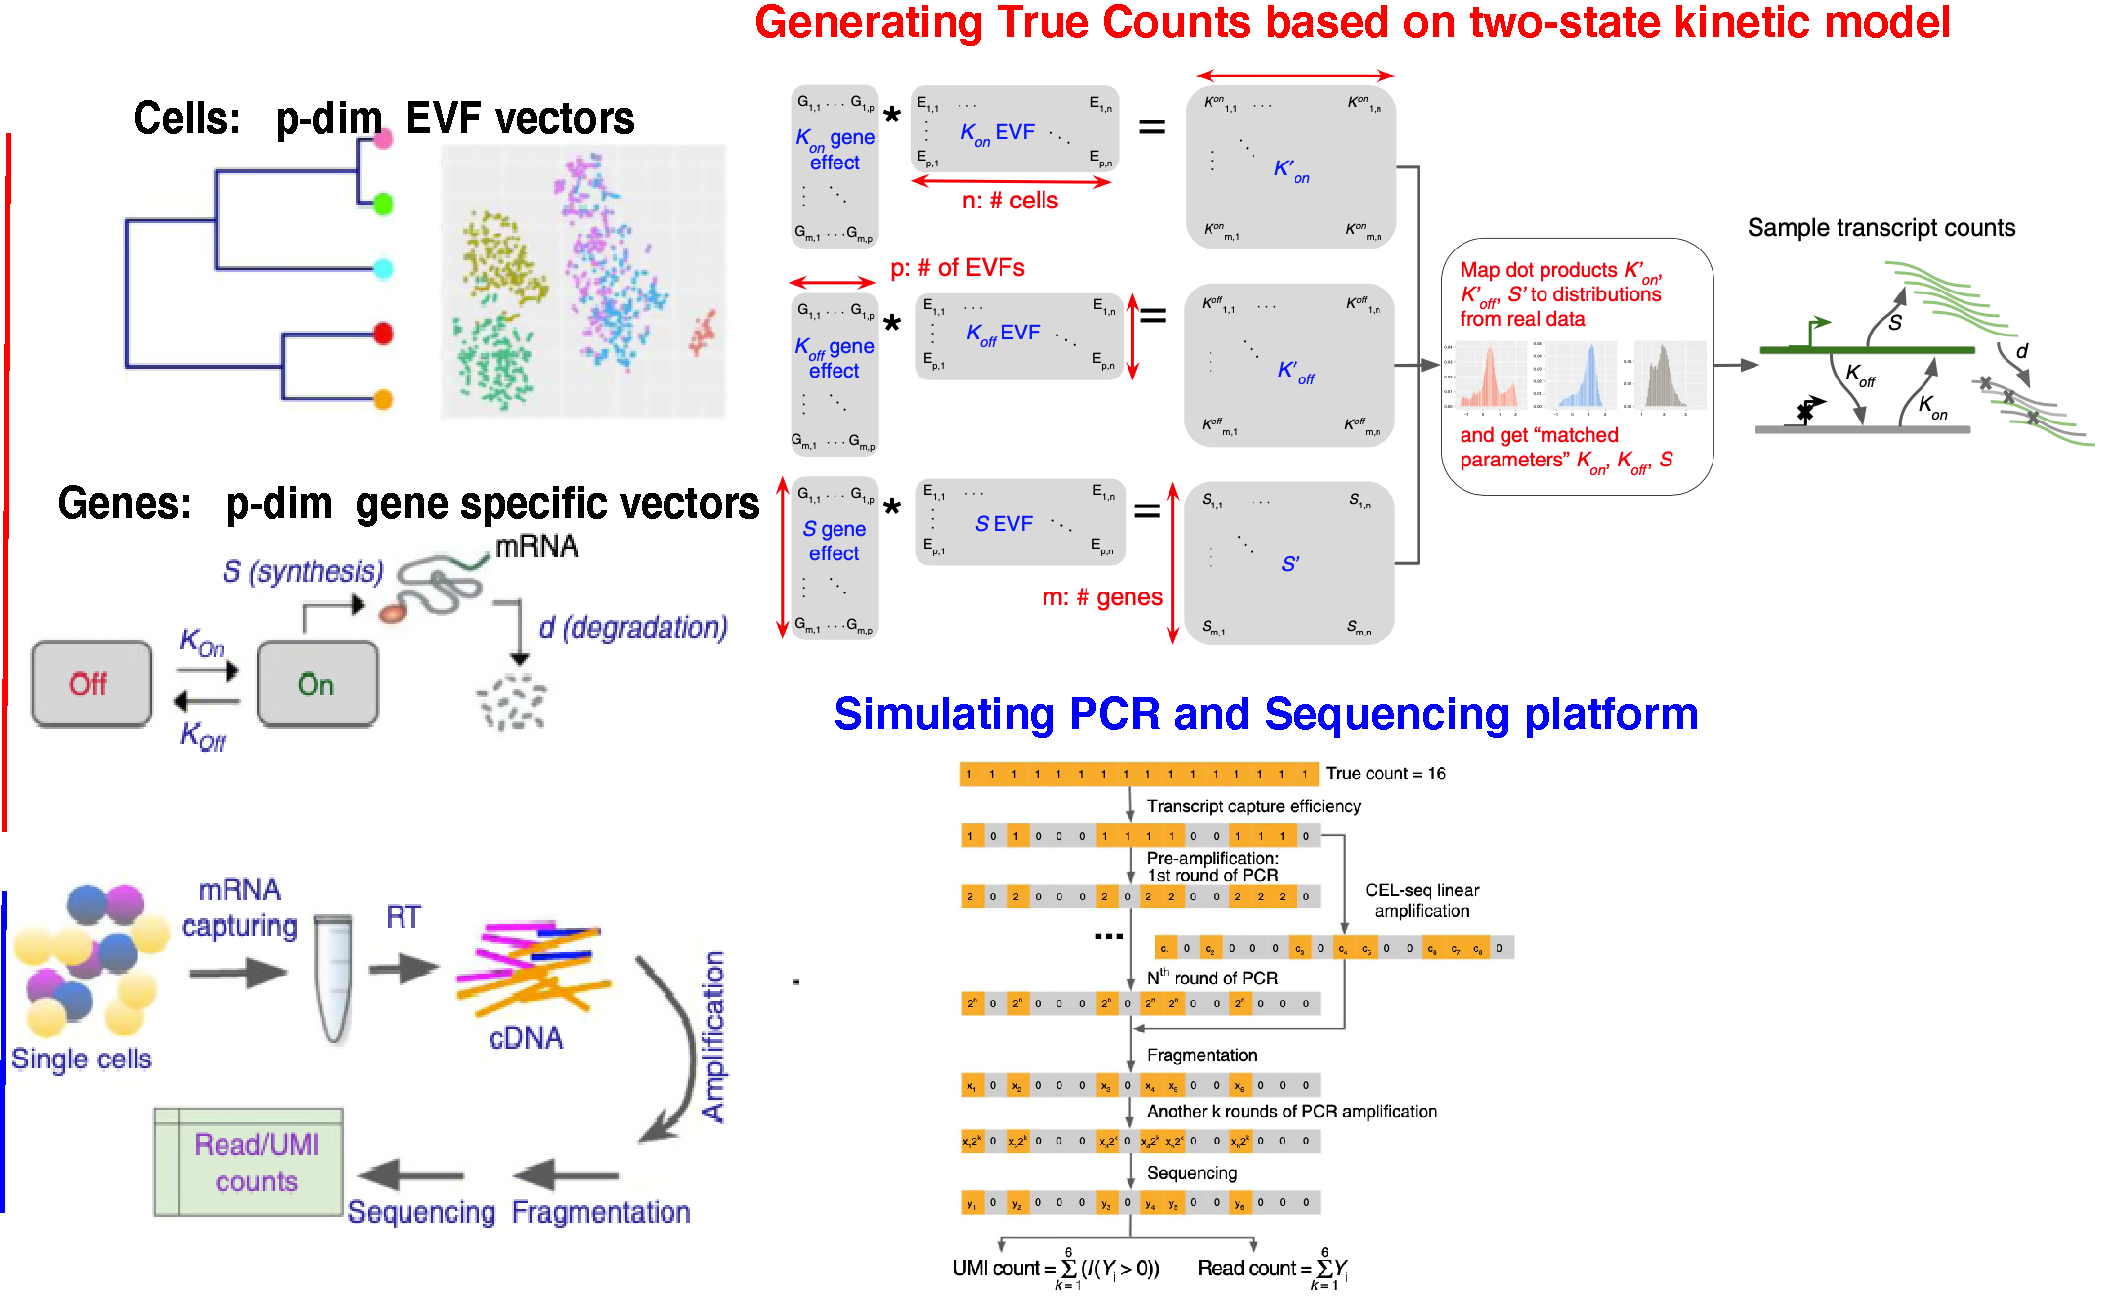
\includegraphics[width=\textwidth]{mssc-symsim}
    \caption{SymSim Overview (\cite{zhang2019simulating})}
  \end{figure}
\end{frame}

\begin{frame}
  \begin{figure}
    \centering
    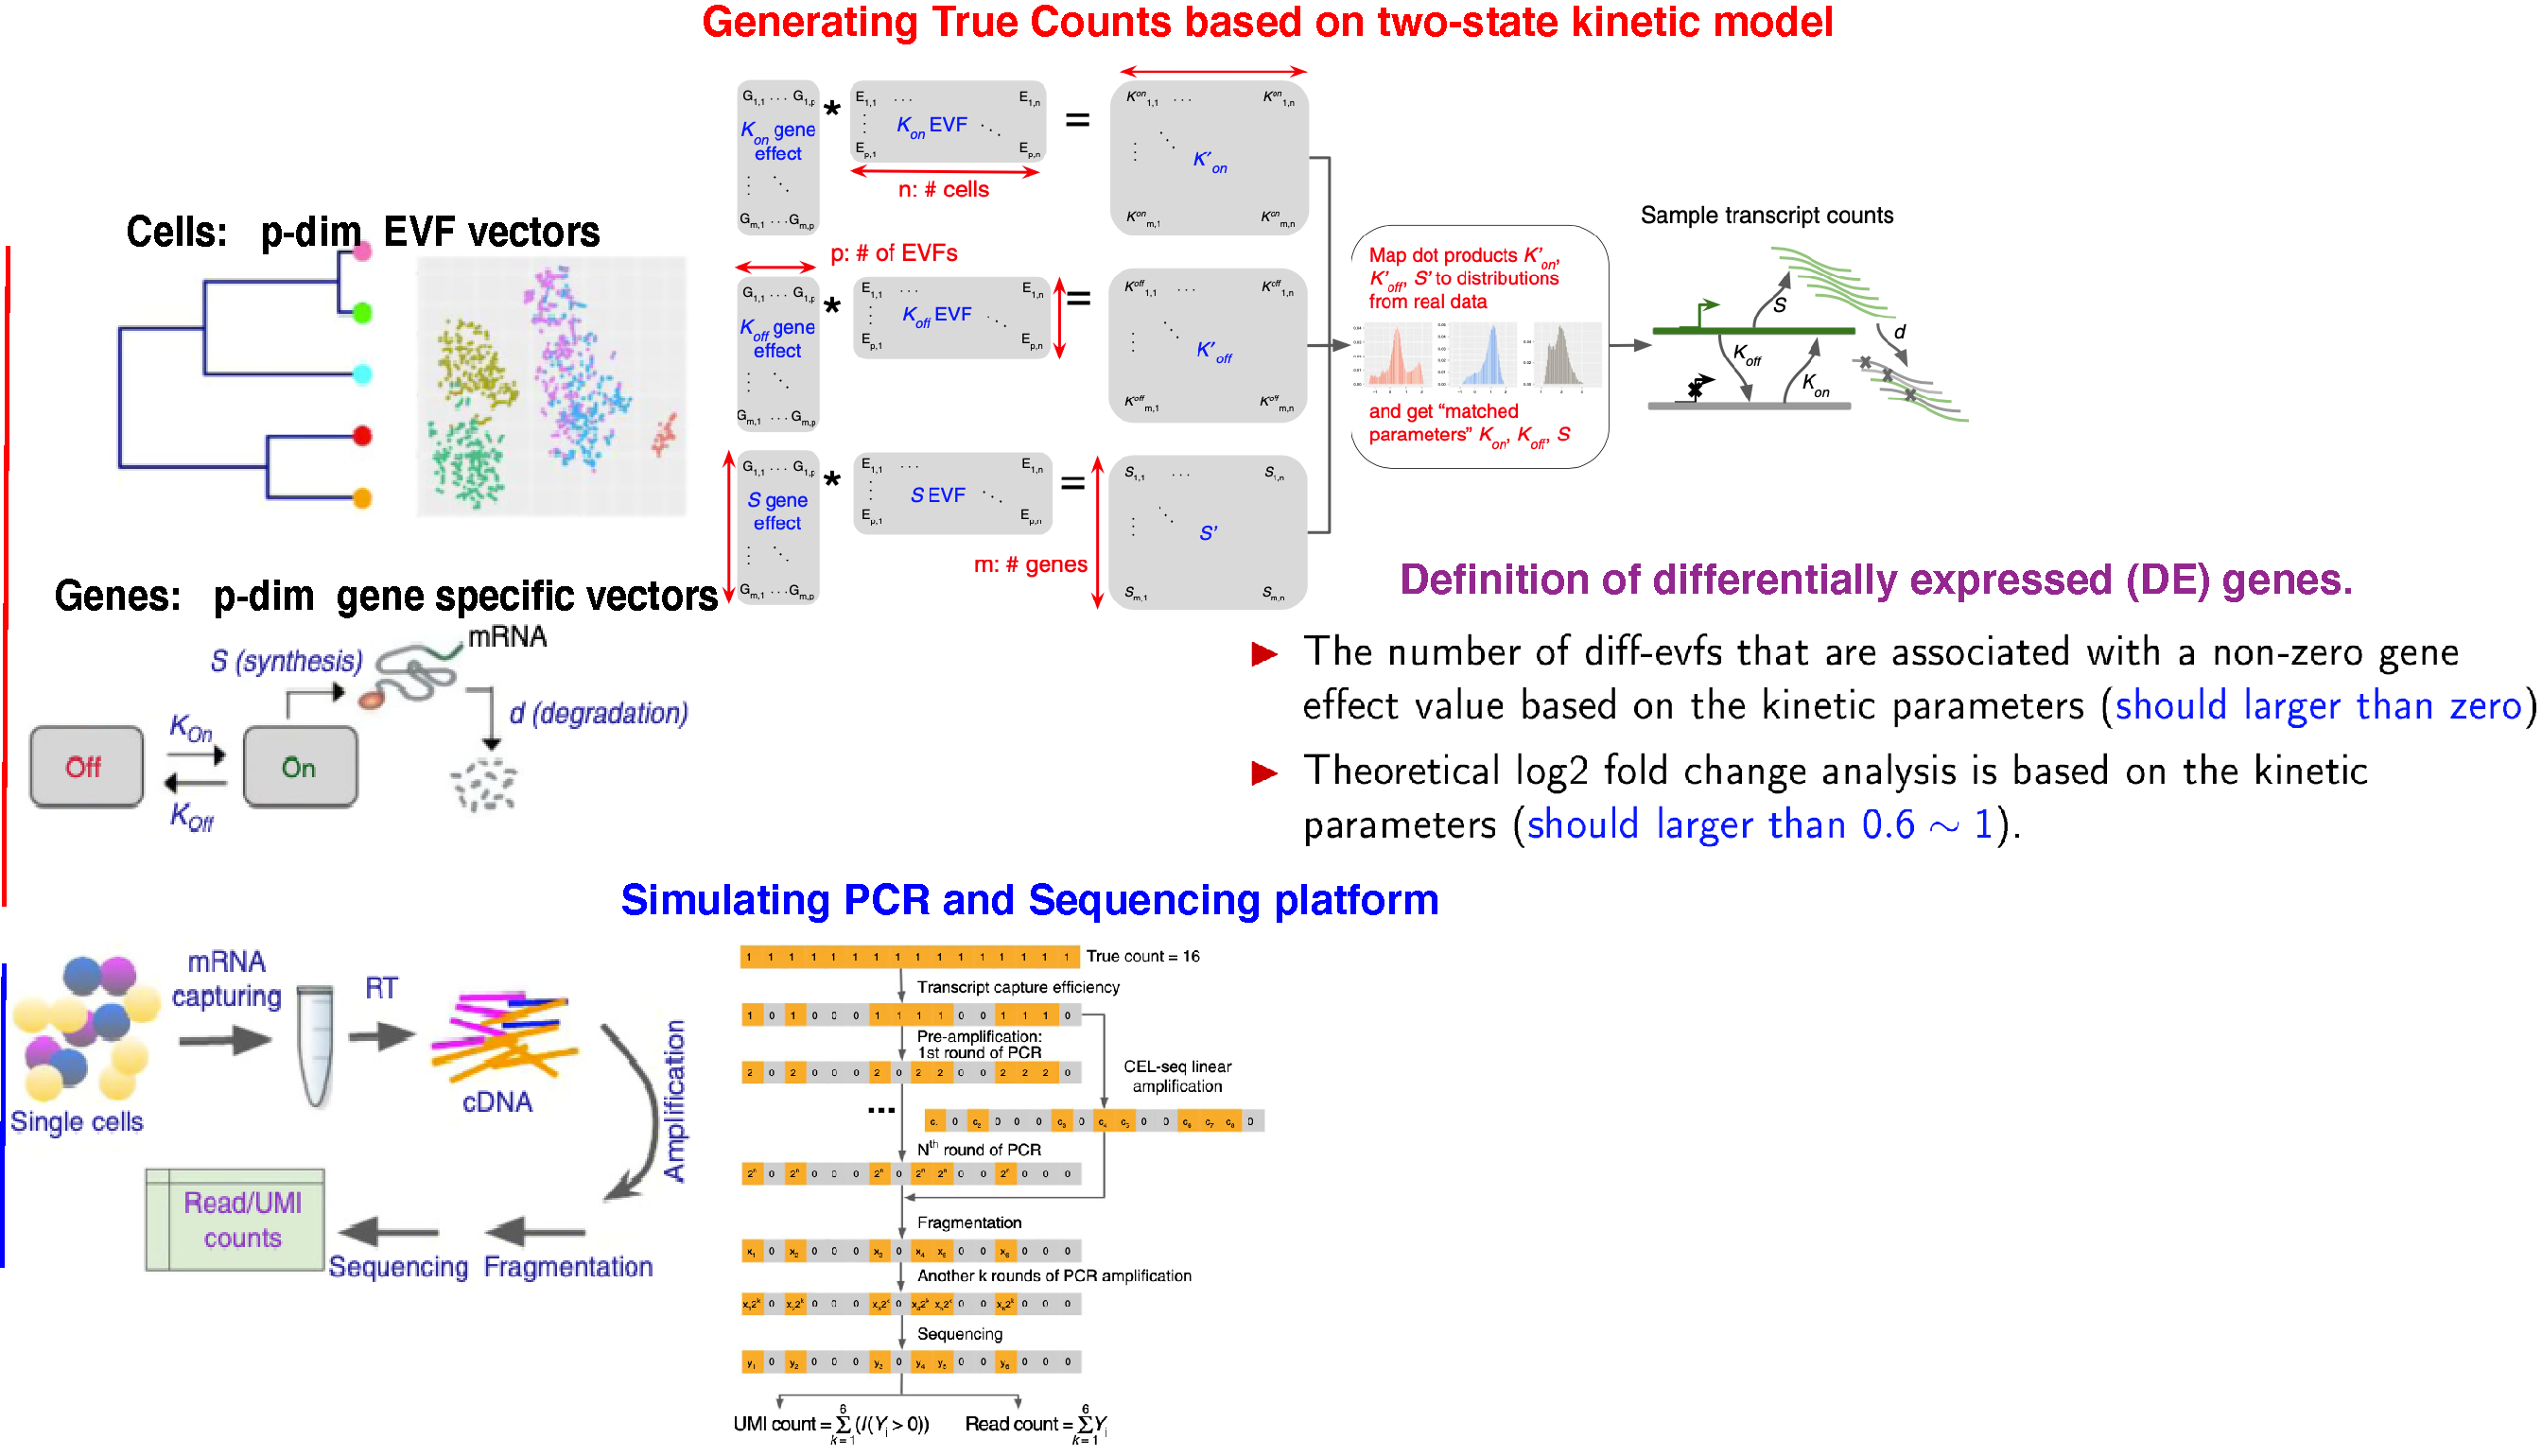
\includegraphics[width=\textwidth]{mssc-symsim_diffgene}
    \caption{DE analysis in SymSim}
  \end{figure}
\end{frame}

\begin{frame}
  \begin{figure}
    \centering
    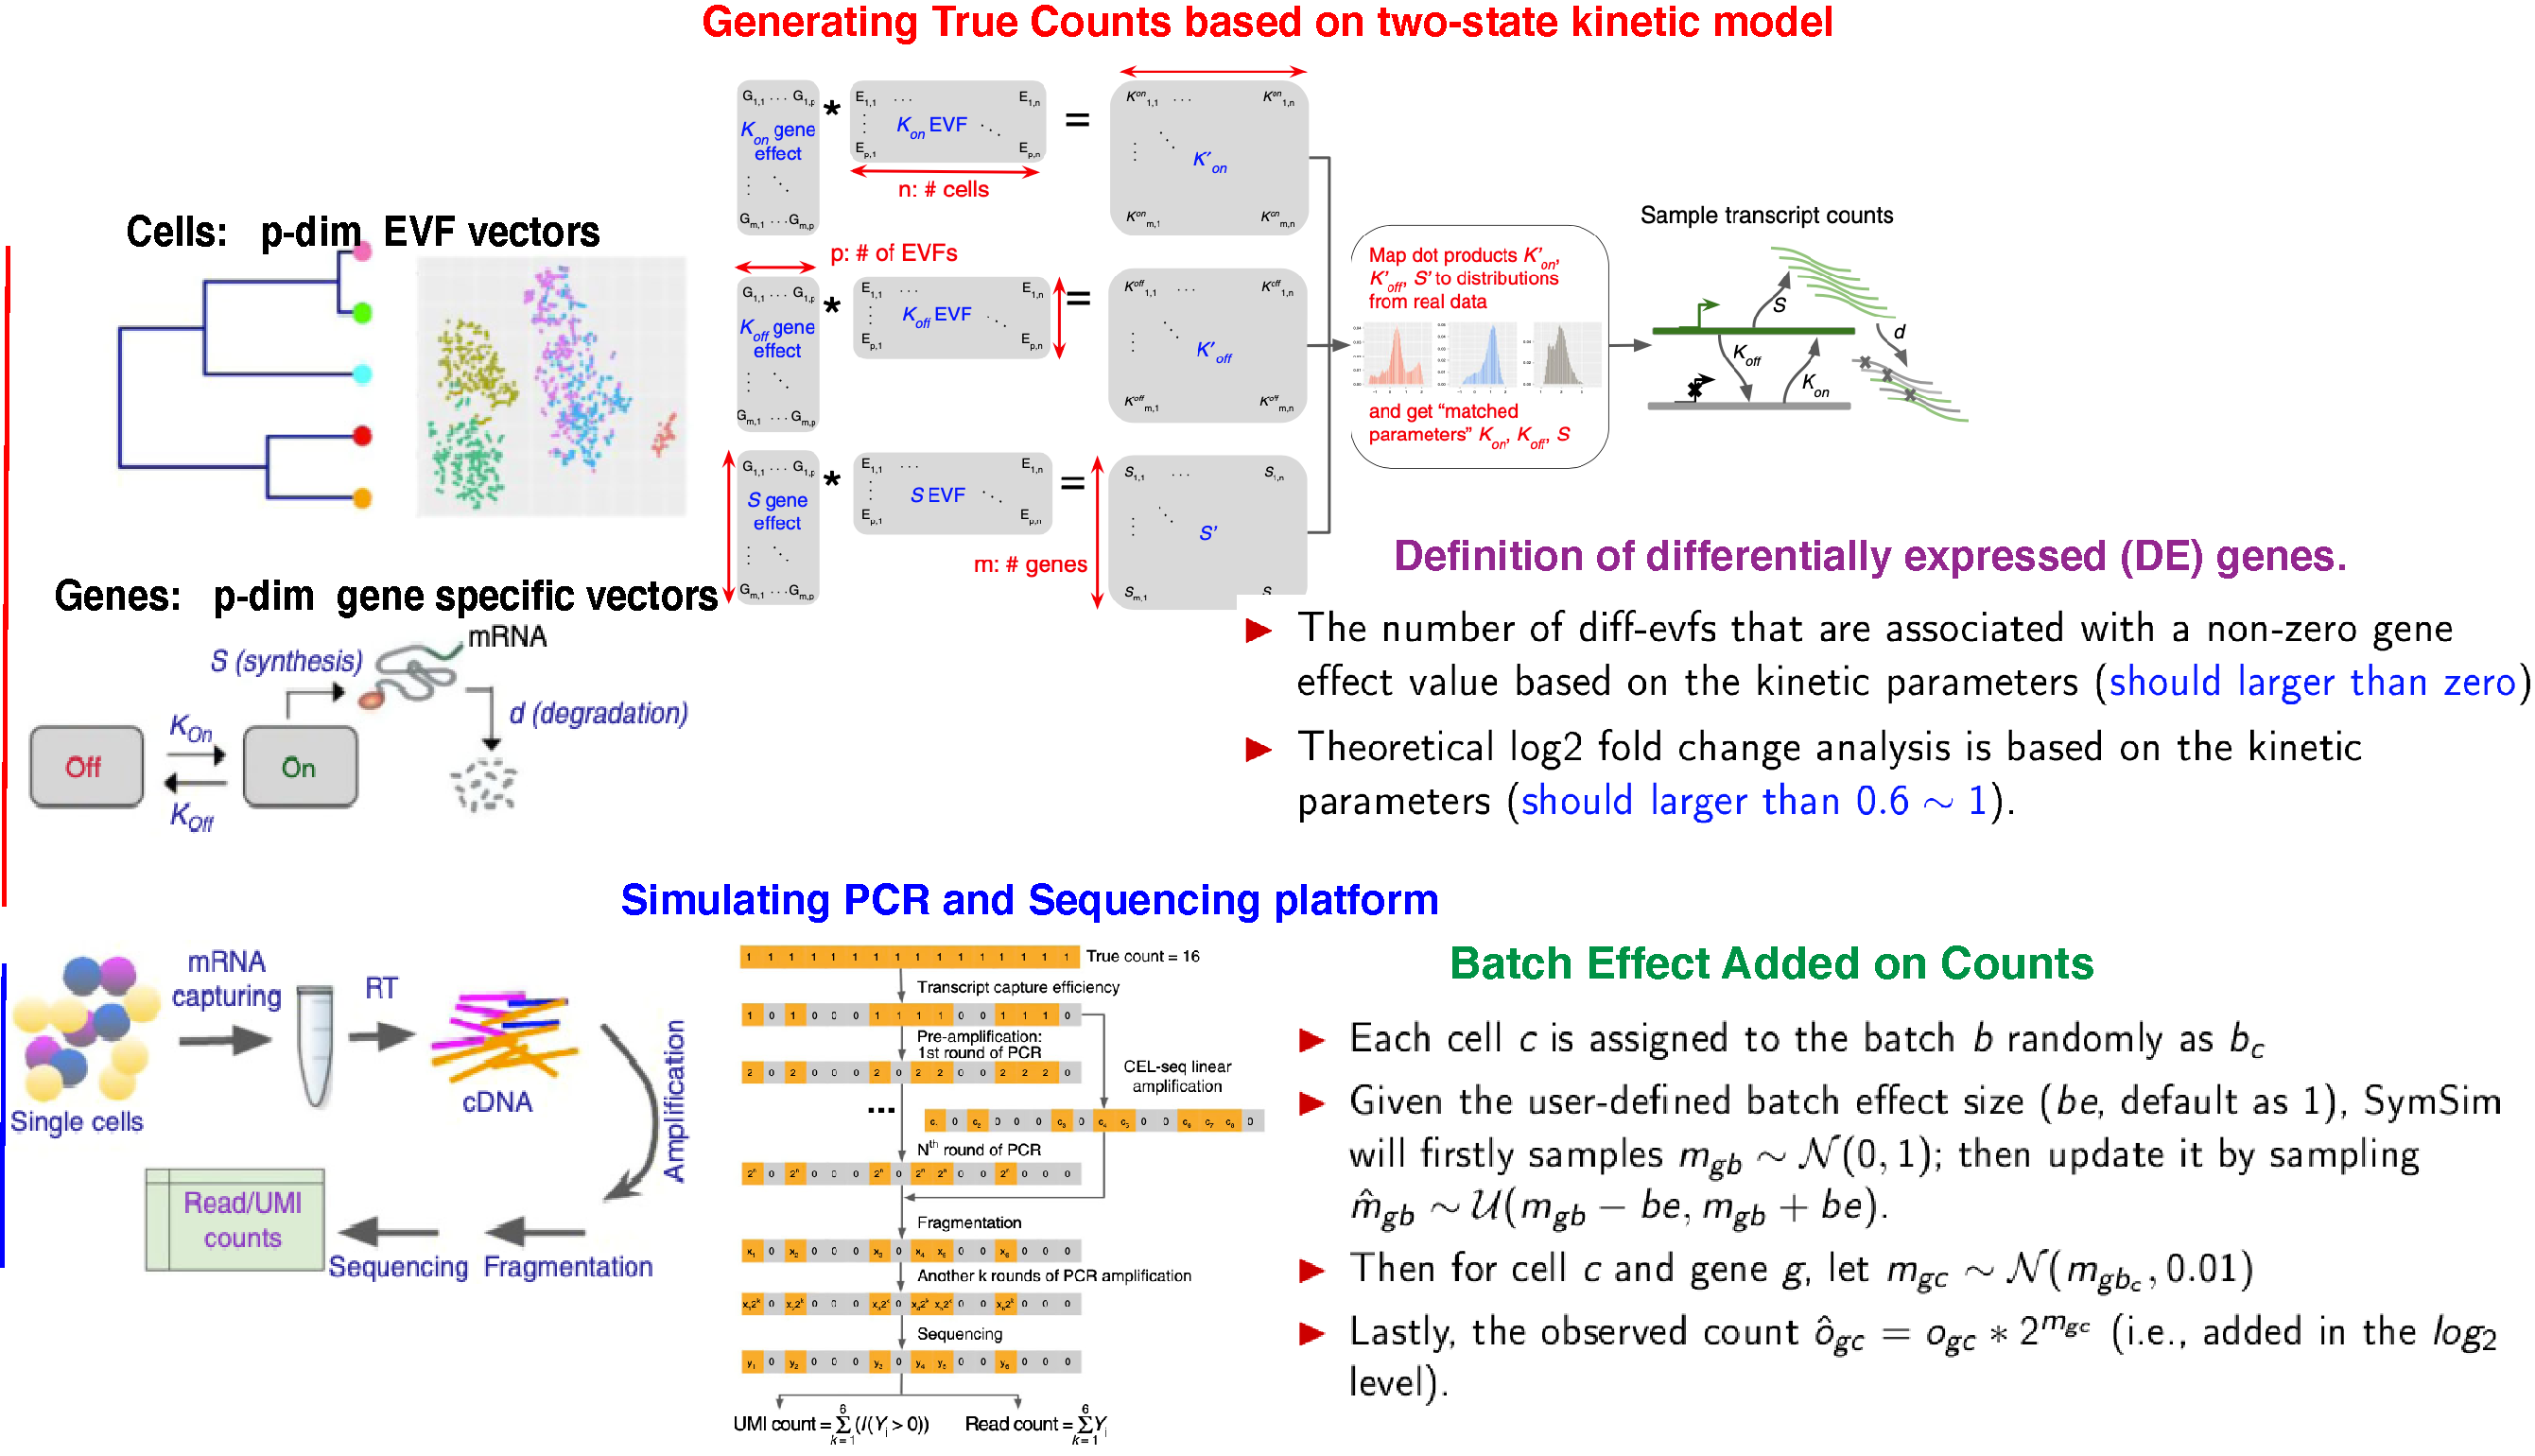
\includegraphics[width=\textwidth]{mssc-symsim_batcheffect}
    \caption{Batch effect in SymSim}
  \end{figure}
\end{frame}

\subsection*{MSSC SymSim}
\begin{frame}
  \frametitle{Simulation based on SymSim}
  \begin{itemize}
  \item
    2000 cells, 300 genes, 10 batch (individuals)
    \begin{itemize}
    \item
      Each individual (ind): about 200 cells
    \item
      \mywarn{Condition 1: Ind 1 to 5 } {\it v.s.} \myemph{Condition 2: Ind 6 to 10}
    \item
      Use the \myemph{two-leaf} phylo-tree, which lets SymSim to generate two cell populations
      as one cell type in two conditions in MSSC.
    \item
      1000 cells in each condition
    \end{itemize}
  \item
    Batch effect added in two sequential steps:
    \begin{enumerate}
    \item
      The default SymSim strategy to add both gene and
      individual-specific batch effect.
    \item
      Sample some non-differential expressed genes, add strong batch effect
      sizes for 1, 2 and 6 to simulate the biased response. {\it For
        instance, in our simulation, \mywarn{71} DE genes, and \mywarn{34}
      \myemph{strictly} non-DE genes. We sample \mywarn{20} genes from the
      strictly non-DE genes in the second step.} 
    \end{enumerate}
  \end{itemize}
\end{frame}

\begin{frame}
  \frametitle{DE genes when no batch effect}
  \begin{figure}
    \centering
    \includegraphics[width=\textwidth]{sample_umi_deg_1}
    \caption{Before batch effect: DE genes} 
  \end{figure}
\end{frame}

\begin{frame}
  \frametitle{non-DE genes when no batch effect}
  \begin{figure}
    \centering
    \includegraphics[width=\textwidth]{sample_umi_ndeg_1}
    \caption{Before batch effect: non-DE genes} 
  \end{figure}
\end{frame}

\begin{frame}
  \frametitle{DE genes after the first batch effect}
  \begin{figure}
    \centering
    \includegraphics[width=\textwidth]{sample_be_deg_1}
    \caption{First batch effect: DE genes} 
  \end{figure}
\end{frame}

\begin{frame}
  \frametitle{Non-DE genes after the first batch effect}
  \begin{figure}
    \centering
    \includegraphics[width=\textwidth]{sample_be_ndeg_1}
    \caption{First batch effect: non-DE genes} 
  \end{figure}
\end{frame}

\begin{frame}
  \frametitle{DE genes after the second batch effect}
  \begin{figure}
    \centering
    \includegraphics[width=\textwidth]{sample_2be_deg_1}
    \caption{Second batch effect: DE genes} 
  \end{figure}
\end{frame}

\begin{frame}
  \frametitle{Non-DE genes after the second batch effect}
  \begin{figure}
    \centering
    \includegraphics[width=\textwidth]{sample_2be_ndeg_1}
    \caption{Second batch effect: non-DE genes} 
  \end{figure}
\end{frame}

\subsection*{Gene-wise batch effect model}
\begin{frame}
  \frametitle{Result Summary based on the AUC}
  \begin{itemize}
  \item
    Both MCMC and VI shows almost the same result.
  \item
    Model v1-1 and v1-2 shows almost the same result, but v1-2 is more
    robustness than v1-1.
  \item
    On the simulation data set, pseudobulk is better than mssc (0.75 vs 0.72). 
  \end{itemize}
\end{frame}

\begin{frame}{Posterior t statistics vs p-value from DESeq2}
  \begin{figure}
    \centering
    \includegraphics[width=\textwidth]{p_v1-1_deg}
    \caption{DE genes: mssc vs pseudo} 
  \end{figure}
\end{frame}

\begin{frame}{Posterior t statistics vs p-value from DESeq2}
  \begin{figure}
    \centering
    \includegraphics[width=\textwidth]{p_v1-1_ndeg}
    \caption{Non-DE genes: mssc vs pseudo}
  \end{figure}
\end{frame}
